\section{The meaning of Necessity}
\label{s:semantics}

In the introduction we spoke of \emph{Necessity Specifications}, e.g., $\onlyIf {A_1} {A_2} {A_3}$. 
% There are three, related, forms of necessity specifications, i.e. $\onlyIf {A_1} {A_2} {A_3}$,
% $\onlyIf {A_1} {A_2} {A_3}$, and 
% $\onlyThrough {A_1} {A_2} {A_3}$, $\onlyIf {A_1} {A_2} {A_3}$.
In this section we will define the semantics of such specifications.
In order to do that, we first define 
an underlying programming language \Loo, (Section \ref{sub:Loo}).
We then  define an assertion language, \SpecO,  which can talk about
 the contents of the state, as well about 
  of provenance and permission(Section \ref{sub:SpecO}).
Finally, we define necessity specifications in \Chainmail (Section \ref{s:holistic-guarantees}).



\subsection{\Loo}
\label{sub:Loo} 
% We introduce a simple object-oriented language, \Loo, upon 
% which our specification language sits.
 \Loo is a small, simple, imperative,
class based, object oriented language. 
Given the simplicity of \Loo, we do not
define it here, \sd{instead,} we direct the reader to Appendix \ref{app:loo} for 
the full \sd{definitions}. % syntax and operational semantics.
\sd{Here we outline the definitions, and  introduce the concepts most relevant to the
treatment of the open world guarantees.}

A \Loo configuration $\sigma$ consists of a 
heap $\chi$, and a frame stack $\psi$ --
\sd{the latter is a sequence of
frames}.    
A frame $\phi$ consists of
local variable map, and \sd{a continuation}, i.e. a sequence of statements to be executed.
 A statement may \sd{assign to variables}, create new objects and push them to the heap, 
perform field reads and writes on objects,  \sd{or}
 call methods on those objects. 

%Program 
\sd{Execution} is performed in the context of a module $M$,
which is a mapping
\sd{from} class names to class definitions. 
\sd{Execution has the format}  $M, \sigma \leadsto \sigma'$, and is
unsurprising,  c.f. Appendix \ref{app:loo}.
\sd{The statements being executed are those in the continuation of the top frame.}
 % chopped, as generic 
 % There are several properties  of \Loo that are important to the central topic of this paper. 
 
\sd{As we said in section \ref{s:approach}, we are interested in guarantees which hold
when the external module is executing, and are not concerned if the internal module xtemporarily
breaks them. Therefore, we are only interested in states where the
executing object (the \prg{this}) is an internal object. 
For this, we define the  \emph{external state semantics}, of the form 
$\reduction{M_1}{M_2}{\sigma}{\sigma'}$, where $M_1$ is the external
module, and $M_2$ is the internal module, and where we
collapse all internal steps into one single step.  }

 
% SD removed, as disagreed with some of what is said below
% which allow us to 
%we define two forms of the operational semantics for \Loo, one in Fig. \ref{f:loo-semantics}
%that is unsurprising and details the execution of specific 
%statements in the language, and a second called \emph{external state semantics} 
%that models that open world, where the components of a program can
%have both known (\internalO) and unknown (\externalO) provenance.

\begin{definition}[External State Semantics]
\label{def:pair-reduce}
For  
% If we say "internal module", it is sounds as something makes the module be internal
  modules $M_1$,  $M_2$, and program configurations $\sigma$, $\sigma'$, 
we say that $\ \ \ \ \ \ \ \ \reduction{M_1}{M_2}{\sigma}{\sigma'}\ \ \ \ \ \ \ \ $ if and only if there exists a 
$n\in\mathbb{N}$, such that
\begin{itemize}
% SD changed because the old version was slightly wrong
\item
\sd{$\sigma$=$\sigma_1$, and  $\sigma'$=$\sigma_n$},
\item
$M_1 \circ M_2, \sigma_i \leadsto \sigma_{i+1}$  \ \ \ for all $i\in [0..n)$,
\item
$\class{\sigma}{\sigma.\prg{this}}, \class{\sigma'}{\sigma'.\prg{this}}\in M_2$,
\item
$\class{\sigma_i}{\sigma_i.\prg{this}} \in M_1$\ \ \ for all $i\in [1..n)$.
\end{itemize} 
%$M_1 \circ M_2, \sigma \leadsto \sigma_1 \leadsto \ldots \sigma_n \leadsto \sigma'$ and $\class{\sigma_i}{\sigma_i.\prg{this}} \in M_1$ for all $0 \leq i \leq n$
%
%$\class{\sigma}{\sigma.\prg{this}}\ \in\ M_2$ and
%\item
%$\class{\sigma'}{\sigma'.\prg{this}}\ \in\ M_2$ and 
%\end{itemize} 
%%and
%%\begin{itemize}
%%\item
%%$\exec{M_1\ \circ\ M_2}{\sigma}{\sigma'}$ or
%%\item
%$M_1 \circ M_2, \sigma \leadsto \sigma_1 \leadsto \ldots \sigma_n \leadsto \sigma'$ and $\class{\sigma_i}{\sigma_i.\prg{this}} \in M_1$ for all $0 \leq i \leq n$
%\end{itemize}
\end{definition}
\begin{figure}[htb]
  \vspace*{-2.5mm}
  \begin{center}
   \begin{minipage}{0.80\textwidth}
     \begin{center}
       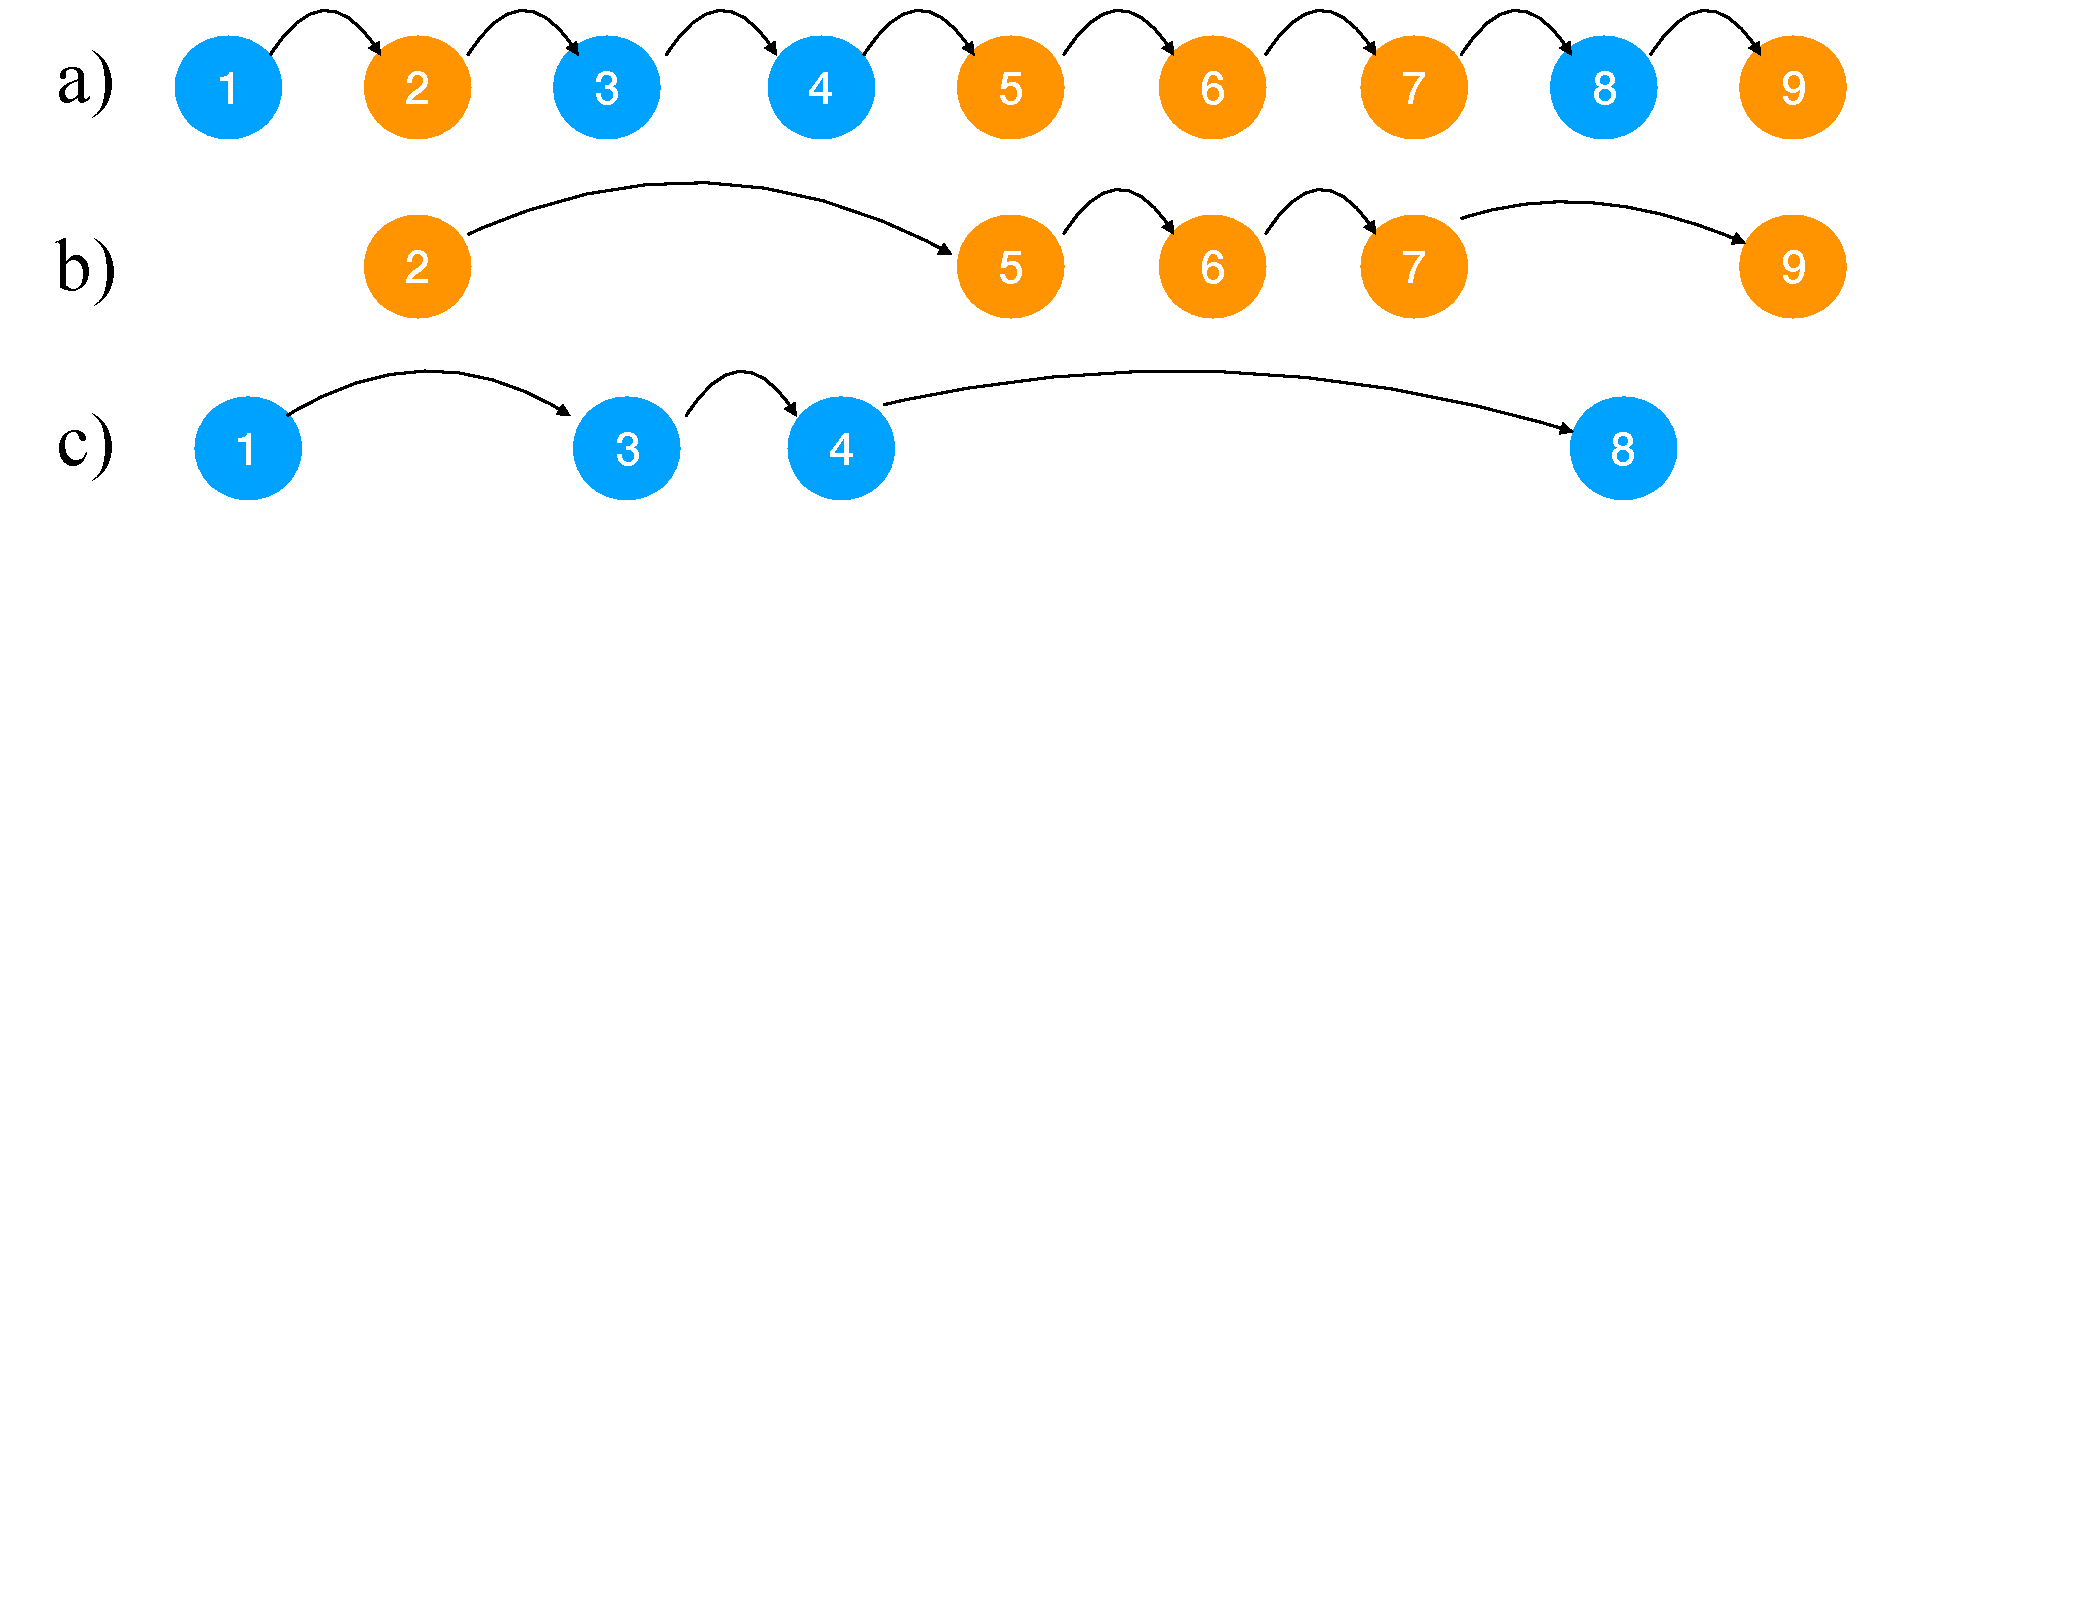
\includegraphics[width=\linewidth]{diagrams/VisibleStates.pdf}
     \end{center}
   \end{minipage}
   \end{center}
   \vspace*{-2.5mm}
   \caption{External State Semantics
     (Def. \ref{def:pair-reduce}). %
     % 
     (a) $\exec{{\color{blue}M_1} \circ {\color{orange}M_2}}{\sigma_1}{\ldots}\leadsto \sigma_9$
     (b) $\reduction{{\color{blue}M_1}}{{\color{orange}M_2}}{\sigma_2}{\ldots}\leadsto \sigma_9$
     (c) $\reduction{{\color{orange}M_2}}{{\color{blue}M_1}}{\sigma_1}{\ldots}\leadsto \sigma_8$
    }
   \label{fig:VisibleStates}
 \end{figure}
\jm[]{
Fig. \ref{fig:VisibleStates} provides a simple graphical description of 
our external state semantics.
}



In the  definition above % of external state semantics makes reference to a 
we \sd{use  the function
$\class{\sigma}{\alpha}$. This function looks up 
the class of the address $\alpha$ in the heap of $\sigma$.} 
  % for a specific variable in a specific program.
% SD not a variable, and no program.
We also use module linking, $M_1\circ M_2$. The operator $\circ$
 %  results in the union of two disjoint modules.
\sd{combines the two modules into one module in the obvious way, provided that their 
domains are disjoint.}
Full details in  Appendix \ref{app:loo}.


\sd{In this work we are interested in guarantees which are upheld by the internal 
module. Therefore, these guarantees  need to be satisfied only at `reachable' states,
and need not be satisfied at states that are
not reachable -- this is described formally in Definition \ref{def:all-sat}. 
Reachable states are those that  may arise by external states execution.
We describe the states of interest as the \emph{arising configurations}. }
\sophia[Here we say why we need Arising. Can you guys say more eloquenlty? Perhaps take from FASE?]{}


% SD thinks that the below is "mechanics" bu we need "intention"
% and I tried to give intention. above
% An \emph{Arising} program configuration is defined as any program configuration
% that arises from some initial program configuration through external state semantics.
\begin{definition}[Arising Program Configuration]
\label{def:arising}
For   modules $M_1$ and  $M_2$, a program configuration $\sigma$ is 
said to be an \emph{arising} configuration, formally \ \ \ $\arising{M_1}{M_2}{\sigma}$,\ \ \ 
if and only if there exists some $\sigma_0$ such that $\initial{\sigma_0}$ and
$\reductions{M_1}{M_2}{\sigma_0}{\sigma}$.
\end{definition}

% Definition \ref{def:arising} uses the definition for 
In the definition above we used \emph{Initial} configurations, 
% he definition of which can be found in  Definition \ref{def:initial}. 
\sd{which are meant to characterise configurations at the start of program execution}.
The heap of an initial configuration should  contain a single object of class \prg{Object}, and
the  stack should consists of a single frame, whose local variable map contains only the 
mapping of \prg{this} to the single object, and whose continuation may be any statement.
% to be executed.
More in Definition \ref{def:initial}. 

%Finally, we assume that there is some type system defined for \Loo that enforces 
%two encapsulation properties:
%\begin{itemize}
%\item
%Classes may be optionally annotated as \enclosed, and objects of \enclosed classes
%may not be returned as method results from non-\enclosed objects
%\item
%Ghost fields may be optionally annotated as \prg{intrnl}, meaning only references to objects 
%internal to the defining module may be used in the definition of that ghost field.
%\end{itemize}
%We do not define this type system for two reasons: (1) such a type system is fairly straightforward
%in it's definition, and largely orthogonal to the central topic of this paper, and (2) while we
%specify a type system, we are only interested in the encapsulation properties that it affords,
%and there are several other equally appropriate mechanisms able to provide such encapsulation 
%properties.


\subsection{\SpecO}
\label{sub:SpecO}
\SpecO extends expressiveness of standard specification languages
with assertion forms capturing key concepts of software security:
 \emph{permission}, \sd{\emph{provenance}}, and \emph{control}.
%That is, \SpecO specifications are able to specify which objects have
%access to which other object (\emph{permission}), whether an object's origin
%is internal or external to known code (\emph{viewpoint}), or which objects call which 
%methods (\emph{control}). 

\subsubsection{Syntax}

\begin{figure}[t]
\footnotesize
\[
\begin{syntax}
\syntaxElement{A}{}
		{
		\syntaxline
				{e}
				{e : C}
				{\neg A}
				{A\ \wedge\ A}
				{A\ \vee\ A}
				{\all{x}{A}}
				{\ex{x}{A}}
		\endsyntaxline
		}
		{
		\syntaxline
				{\access{x}{y}}
				{\internal{x}}
				{\external{x}}
		\endsyntaxline
		}
		{
		\syntaxline
				{\calls{x}{y}{m}{\overline{z}}}
		\endsyntaxline
		}
\endSyntaxElement\\
\end{syntax}
\]
\caption{\SpecO Assertions}
\label{f:chainmail-syntax}
\end{figure}



Fig. \ref{f:chainmail-syntax} gives the assertion syntax of the \SpecO specification language.
An assertion may be an expression, a class assertion, the usual connectives and quantifiers, along 
with several non-standard assertion forms:
\begin{itemize}
\item
\emph{Permission} ($\access{x}{y}$): % Which objects have access to which other objects (i.e.
  \sd{$x$ has access to $y$}.
\item
{\emph{Provenance}} ($\internal{x}$ and $\external{y}$): %Which objects are internal or external to our component.
 \sd{$x$ is internal, and $y$ is external}.
\item
\emph{Control} ($\calls{x}{y}{m}{\overline{z}}$): 
\sd{$x$ calls method $m$ on object $y$ with arguments $\overline{z}$}.
\end{itemize}

\subsubsection{Semantics of \SpecO}
The semantics of \SpecO assertions is given in Definition \ref{def:chainmail-semantics}. 
The definition of the semantics of \SpecO makes use of several language features of 
\Loo that can be found in Appendix \ref{app:loo}. Specifically, $\eval{M}{\sigma}{e}{v}$
is the evaluation relation for expressions, and is interpreted as expression $e$ evaluates
to value $v$ in the context of program configuration $\sigma$, with module $M$. The full
semantics of expression evaluation are given in Fig. \ref{f:evaluation}. It should 
be noted that expressions in \Loo may be recursively defined, and thus evaluation may not
necessarily terminate, however the logic remains classical because recursion is restricted
to expressions, and not generally to assertions.

Further, Definition \ref{def:chainmail-semantics} uses the interpretation of variables
within a specific frame or configuration: i.e. $\interpret{\phi}{x} = v$, meaning that $x$ maps to
value $v$ in the local variable map of frame $\phi$, and $\interpret{\sigma}{x} = v$ meaning $x$ 
maps to value $v$ in the top most frame of $\sigma$'s stack.

\begin{definition}[Satisfaction of \SpecO Assertions] 
\label{def:chainmail-semantics}
We define satisfaction of an assertion $A$ by a program configuration $\sigma$ with internal module $M$ as:
\begin{itemize}
\item
$\satisfiesA{M}{\sigma}{e}$ \ \ \ iff \ \ \  $\eval{M}{\sigma}{e}{\true}$
\item
$\satisfiesA{M}{\sigma}{e : C}$ \ \ \ iff \ \ \  $\eval{M}{\sigma}{e}{\alpha}$ \textit{and} $\sigma.\prg{heap}(\alpha).\prg{class} = C$
\item
$\satisfiesA{M}{\sigma}{\neg A}$ \ \ \ iff \ \ \  ${M},{\sigma}\nvDash{A}$
\item
$\satisfiesA{M}{\sigma}{A_1\ \wedge\ A_2}$ \ \ \ iff \ \ \  $\satisfiesA{M}{\sigma}{A_1}$ and 
$\satisfiesA{M}{\sigma}{A_2}$
\item
$\satisfiesA{M}{\sigma}{A_1\ \vee\ A_2}$ \ \ \ iff \ \ \  $\satisfiesA{M}{\sigma}{A_1}$ or 
$\satisfiesA{M}{\sigma}{A_2}$
\item
$\satisfiesA{M}{\sigma}{\all{x}{A}}$ \ \ \ iff \ \ \  
\sd{$\satisfiesA{M}{\sigma[x \mapsto \alpha]}{A}$, \ 
\ \ for some $x$ fresh in $\sigma$, and for all $\alpha\!\in\!\sigma.\prg{heap}$. } 
\footnote{used to say: $\satisfiesA{M}{\sigma'}{A}$, 
where $x$ is fresh in $\sigma$ and $\sigma' = \sigma[x \mapsto \alpha]$, 
for all $\alpha \in \sigma.\prg{heap}$
\\
but this feels wrong -- things introduced in wrong order}
\item
$\satisfiesA{M}{\sigma}{\ex{x}{A}}$ \ \ \ iff \ \ \  
\sd{$\satisfiesA{M}{\sigma[x \mapsto \alpha]}{A}$, \ 
\ \ for some $x$ fresh in $\sigma$, and for some $ \alpha\!\in\!\sigma.\prg{heap}$. } 
\footnote{used to say: $\satisfiesA{M}{\sigma}{A}$ \\
where $x$ is fresh in $\sigma$ and $\sigma' = \sigma[x \mapsto \alpha]$
for some $\alpha \in \sigma.\prg{heap}$}
\item
$\satisfiesA{M}{\sigma}{\access{x}{y}}$ \ \ \ iff \ \ \  
\begin{itemize}
\item
\footnote{used to say: $\exists\ f$ such that $\interpret{\sigma}{x.f}={\interpret{\sigma}{y}}$ ... :-(}
$\interpret{\sigma}{x.f}={\interpret{\sigma}{y}}$ \sd{for some $f$}, \  or
\item
there exists some $z$, and some frame $\phi$ in the stack of $\sigma$ such that $\interpret{\phi}{x}=\interpret{\phi}{\prg{this}}$ 
% and there exists such that $\interpret{\phi}{y}=\interpret{\phi}{z}$
\end{itemize}
\item
$\satisfiesA{M}{\sigma}{\internal{x}}$ \ \ \ iff \ \ \  
$\textit{classOf}(\sigma,x) \in M$
\item
$\satisfiesA{M}{\sigma}{\external{x}}$ \ \ \ iff \ \ \  
$\textit{classOf}(\sigma,x) \not\in M$
\item
$\satisfiesA{M}{\sigma}{\calls{x}{y}{m}{z_1, \ldots, z_n}}$ \ \ \ iff \ \ \ 
\begin{itemize}
\item
$\sigma.\prg{contn} = (\_ := y'.m(z'_1,\ldots,z'_n))$, % and is superfluous, enums are ands, unless expltly stated   
\item
$\interpret{\sigma}{x} = \interpret{\sigma}{\prg{this}}$  % and
\item
$\sd{\interpret{\sigma}{y} = \interpret{\sigma}{y'}}$ % and
\item
$\interpret{\sigma}{z_i} = \interpret{\sigma}{z'_i}$ \ \ \ for all $1\!\leq i\!\leq n$
\end{itemize}
\end{itemize}
\end{definition}

\jm[]{
We also define what it means for a module to satisfy an assertion in
Definition \ref{def:mdl-sat}. That is, assertions that are satisfied
by all arising program configurations for a given \internalM module.
\begin{definition} [Assertion Satisfaction by Modules]
\label{def:mdl-sat}
For a module $M$ and assertion $A$, we say that\ \  $\satisfies{M}{A}$ \ \ if and only if 
for all modules $M'$, and all $\sigma$, if $\arising{M'}{M}{\sigma}$, then $\satisfiesA{M}{\sigma}{A}$.
\footnote{used to say: \ \ $\satisfiesA{M}{\sigma}{A}$ for all program configurations $\sigma$. \ \  
but this is wrong }
\end{definition}
Satisfaction by a module is important as it allows us to talk 
about what is true for a given module without introducing the 
details of specific program configurations, a critical component 
of constructing our Logic of Necessity in Section \ref{s:inference}.}

\jm[I have put this here, but I'm not sure it makes sense here ...]{
In order to both define the Logic of Necessity, and construct many proofs of the examples presented in this paper,
we need the ability to reason about \SpecO 
apart from Necessity Specifications. That is, we rely on the existence of
a relation of the form $\proves{M}{A}$. Again, as with encapsulation, this does not fall in the 
domain of our logic of necessity, but is a secondary relation upon which soundness relies. Such a logic is also useful in presenting proofs 
of examples in this paper. For this reason, we elide the definition 
of such a logic, but rely on the existence of one and its soundness. Axiom \ref{ax:specO-prove-soundness}
states our assumption of soundness of such a logic.
\begin{axiom}[Soundness of \SpecO Provability]
\label{ax:specW-prove-soundness}
For all modules $M$ and assertions $A$, $\proves{M}{A}$ then $\satisfies{M}{A}$.
\end{axiom}
}

%\begin{figure}[t]
%\begin{mathpar}
%\infer
%		{M;\ M',\ \sigma\ \vdash\ e : \prg{intrnl}}
%		{M;\ M',\ \sigma\ \vdash\ e : \prg{encap}}
%		\and
%\infer
%		{M;\ M',\ \sigma\ \vdash\ e : \prg{intrnl}}
%		{M;\ M',\ \sigma\ \vdash\ e.f : \prg{encap}}
%		\and
%\infer
%		{M;\ M',\ \sigma\ \vdash\ e : \prg{intrnl}}
%		{M;\ M',\ \sigma\ \vdash\ e.g(e') : \prg{encap}}
%\end{mathpar}
%\caption{Encapsulated Expressions}
%\label{f:intrnl}
%\end{figure}
	
%	\begin{figure}[h]
%	\[
%	\begin{array}{llr}
%	A & ::= & \textit{Assertions}\\  
%	| & e & \\
%	| & e\ :\ C & \\
%	| & e\ \in\ S & \\
%	| & A\ \prg{in}\ S & \\
%	| & \access{x}{y} \\
%	| & \internal{x} \\
%	| & \external{x} \\
%%	| & \mut x y f &\\
%%	| & \gives x y z &\\
%	| & \calls{x}{y}{m}{args} \\
%	| & \changes{S}{A} \\
%	| & \neg A & \\
%	| & A\ \wedge\ A & \\
%	| & A\ \vee\ A & \\
%	| & A\ \longrightarrow\ A & \\
%	| & \forall\ x.\ [A] & \\
%	| & \exists\ x.\ [A] & \\
%	| & \forall\ S.\ [A] & \\
%	| & \exists\ S.\ [A] &
%	\end{array}
%%	\begin{array}{llr}
%%	s & ::= & \textit{Source}\\
%%	| & \prg{int} & \\
%%	| & \prg{ext} & \\
%%	| & \_ &
%%	\end{array}
%	\]
%	\caption{Assertions}
%	\label{f:assertions_triple2}
%	\end{figure}





\subsection{\Chainmail} % \subsection{Necessity Specifications}
\label{s:holistic-guarantees}

In this Section we define syntactic forms and semantics of
\emph{Necessity Specifications}. Fig. \ref{f:holistic-syntax} 
gives the syntax.
\footnote{
Here it used tio say: "We express satisfaction of Necessity Specifications as $\satisfies{M}{H}$.
That is, a module $M$ satisfies a necessity specification $H$. This allows 
the construction of proofs without considering either the details 
of the program configuration or the external client module." But the proofs are
a separate concern than the meaning of H}
We have three forms of Necessity Assertions, described below:

\begin{figure}[t]
\footnotesize
\[
\begin{syntax}
\syntaxElement{H}{}
		{
		\syntaxline
				{\onlyIf{A_1}{A_2}{A_3}}
				{\onlyThrough{A_1}{A_2}{A_3}}
%		\endsyntaxline
%		}
%		{
%		\syntaxline
				{\onlyIfSingle{A_1}{A_2}{A_3}}
		\endsyntaxline
		}
\endSyntaxElement\\
\end{syntax}
\]
\caption{Syntax of \Chainmail}
\label{f:holistic-syntax}
\end{figure}


\jm[wrt. \Chainmail vs \SpecO: I have changed most references to \SpecO, as that was what I meant when I mentioned \Chainmail. I think there may be some mis-renamings though. I will check carefully tomorrow on my read through, but be aware there may be some weird renamings.]{}

\paragraph{Only If}
[$\onlyIf{A_1}{A_2}{A}$]: If an arising program configuration starts at some state $A_1$, and reaches some state $A_2$, 
then the original program state must have also satisfied $A$.
e.g. if the balance of a bank account changes over time, then there must be some external object in the current 
program state that has access to the account's password.

\paragraph{Single-Step Only If}
[$\onlyIfSingle{A_1}{A_2}{A}$]: If an arising program configuration starts at some state $A_1$, and reaches some state $A_2$ after a single execution step, 
then the original program state must have also satisfied $A$.
e.g. if the balance of a bank account changes over a single execution step, then that execution step must be a method call to the bank \prg{transfer} method.

\paragraph{Only Through}
[$\onlyThrough{A_1}{A_2}{A}$]: If an arising program configuration starts at some $A_1$ state, and reaches some $A_2$ state, then program execution must have passed through some $A$ state.
e.g. if the balance of an account changes over time, then the bank's \prg{transfer} method must have been called 
in some intermediate state. Note 
that the intermediate state where $A$ is true might be the initial state ($\sigma_1$),
or final state ($\sigma_2$). 



\jm[]{As programs execute, the local variable 
map may change, variables may be overwritten, or the entire local variable maps may be lost on a method return.
For this reason, before we provide the semantics of Necessity Specifications, we first introduce an adaptation operator
to account for variable renaming throughout the execution of a program.
\begin{definition}
$\adapt{\sigma}{\sigma'} \triangleq (\chi, \{\prg{local} := \beta'[\overline{z}' \mapsto \beta(\overline{z})], \prg{contn}:= [\overline{z}/\overline{z'}]c\} : \psi)$
where 
\begin{itemize}
\item
$\sigma = (\chi, \{\prg{local}:=\beta, \prg{contn}:=c\} : \psi)$ and
$\sigma' = (\_, \{\prg{local}:=\beta'; \prg{contn}:=\_\} : \_)$, and
\item
$dom(\beta) = \overline{z}$, $dom(\beta') \cap \overline{z}' = \emptyset$, and $|\overline{z}| = |\overline{z}'|$
\end{itemize}
\end{definition}}
We define $M \models H$ the semantics of the Necessity Specifications in Definition \ref{def:necessity-semantics}. \sd{The definition goes by cases over the three possible syntactic forms of $H$:}


\noindent
\begin{definition}[Necessity Specifications]
\label{def:necessity-semantics}
For any assertions $A_1$, $A_2$, and $A$,  we define \\

$\bullet$ \ $\satisfies{M}{\onlyIf {A_1}{A_2}{A}}$ \ \ iff\ \  for all $M'$, $\sigma$, $\sigma'$, such that $\arising{M}{M'}{\sigma}$; \\ % and\\

\begin{tabular}{lr}
$\;\;\;\;$- $\satisfiesA{M}{\sigma}{A_1}$  & \rdelim\}{3}{3mm}[$\;\;\;\Rightarrow\;\;\;$  $\satisfiesA{M}{\sigma}{A}$] \\
$\;\;\;\;$- $\satisfiesA{M}{\sigma' \triangleleft \sigma}{A_2}$   \\
$\;\;\;\;$- $\reductions{M}{M'}{\sigma}{\sigma'}$   \\
\end{tabular}\\ 

$\bullet$ \  $\satisfies{M}{\onlyIfSingle {A_1}{A_2}{A}}$\ \ iff\ \   for all $M'$, $\sigma$,   $\sigma'$, such that $\arising{M}{M'}{\sigma}$: \\

\begin{tabular}{lr}
$\;\;\;\;$- $\satisfiesA{M}{\sigma}{A_1}$  & \rdelim\}{3}{3mm}[$\;\;\;\Rightarrow\;\;\;$  $\satisfiesA{M}{\sigma}{A}$] \\
$\;\;\;\;$- $\satisfiesA{M}{\sigma' \triangleleft \sigma}{A_2}$   \\
$\;\;\;\;$- $\reduction{M}{M'}{\sigma}{\sigma'}$   \\
\end{tabular}\\ 

%% here as it was 
%$\bullet$ \  $\satisfies{M}{\onlyThrough {A_1}{A_2}{A}}$ \ \ iff\ \  for all $M'$, $\sigma$,   $\sigma'$, such that $\arising{M}{M'}{\sigma}$, and \\
%\begin{tabular}{lr}
%$\;\;\;\;$- $\satisfiesA{M}{\sigma}{A_1}$  & 
%\rdelim\}{3}{3mm}%[\makecell{Some really \\ longer text}]
%[$\;\;\;\Rightarrow\;\;\;$\pbox{9cm}{then for all $\sigma_1, \ldots, \sigma_n$ such that $\reduction{M}{M'}{\sigma}{\sigma_1}\leadsto \ldots \sigma_n \leadsto \sigma'$
%there exists some $\sigma_i$ such that $\satisfiesA{M}{\sigma_i \triangleleft \sigma}{A}$ where $0\leq i \leq n$, or $\satisfiesA{M}{\sigma}{A}$, or $\satisfiesA{M}{\sigma' \triangleleft \sigma}{A}$}] \\
%$\;\;\;\;$- $\satisfiesA{M}{\sigma' \triangleleft \sigma}{A_2}$   \\
%$\;\;\;\;$- $\reductions{M}{M'}{\sigma}{\sigma'}$   \\
%\end{tabular}\\ 
%$\bullet$ \  $\satisfies{M}{\onlyThrough {A_1}{A_2}{A}}$ \ \ iff\ \  for all $M'$, $\sigma_1$,   $\sigma_n$, such that $\arising{M}{M'}{\sigma}$: \\
  
$\bullet$ \  $\satisfies{M}{\onlyThrough {A_1}{A_2}{A}}$ \ \ iff\ \  for all $M'$, $\sigma_1$,   $\sigma_n$, such that $\arising{M}{M'}{\sigma_1}$: \\

\begin{tabular}{lr}
$\;\;\;\;$- $\satisfiesA{M}{\sigma_1}{A_1}$  & 
\rdelim\}{3}{3mm}%[\makecell{Some really \\ longer text}]
[$\;\;\;\Rightarrow\;\;\;$\pbox{9cm}{$\forall \sigma_2, \ldots, \sigma_{n-1}$.  \\ 
(\ \ $\forall i\!\in\![1..n).\ \reduction{M}{M'}{\sigma_i}{\sigma_{i+1}}$   \ $\Rightarrow$
$\exists i\!\in\![1..n]. \  \satisfiesA{M}{\sigma_n \triangleleft \sigma_1}{A}$ \ \ )   }] \\
$\;\;\;\;$- $\satisfiesA{M}{\sigma_n\triangleleft \sigma}{A_2}$   \\
$\;\;\;\;$- $\reductions{M}{M'}{\sigma}{\sigma_n}$   \\
\end{tabular} 
\end{definition} 

\jm[]{
With the necessity specifications as defined in Definition \ref{def:necessity-semantics},
we are able to state what are the necessary preconditions to critical functions in 
software, including safety properties of software in the open world. The semantics
of \emph{Single-Step Only If} allow for the statement of such necessary preconditions
for any execution step for any program to achieve a certain outcome. The semantics
of \emph{Only If} and \emph{Only Through} allow us to raise these necessary preconditions
to any arbitrary number of execution steps, and thus allow for reasoning about 
the execution of an entire program, even those programs in the open world, where
client functions are unknown and unspecified in a traditional manner.
}

\jm[]{
As an example of how we use necessity specifications, consider the original 
bank account example discussed in Section \ref{s:intro}, we have already shown
how we can reason about knowledge of an account's password using \prg{NecessityBankSpec},
but we are also able to write other useful properties about the bank account. 
}
\begin{lstlisting}[language = Chainmail, mathescape=true, frame=lines]
NecessityBankSpec'  $\triangleq$  from a:Account $\wedge$ a.balance==bal
                       to1 a.balance < bal
                       onlyIf $\exists$ o.[$\external{\texttt{o}}$ $\wedge$ $\calls{\prg{o}}{\prg{a}}{\prg{transfer}}{\prg{\_, \_, \_}}$]
\end{lstlisting}
\jm[]{
\prg{NecessityBankSpec'} states that if over a single step the balance of an account decreases, then it must have occurred as 
a result of a call to \prg{transfer}.
}
\begin{lstlisting}[language = Chainmail, mathescape=true, frame=lines]
NecessityBankSpec''  $\triangleq$  from a:Account $\wedge$ a.password == pwd
                        to a.password != pwd
                        onlyThrough $\exists$ o.[$\external{\texttt{o}}$ $\wedge$ $\calls{\prg{o}}{\prg{a}}{\prg{set}}{\prg{pwd, \_}}$]
\end{lstlisting}
\jm[]{
\prg{NecessityBankSpec''} states that if over an arbitrary number of execution steps, the password of an account changes,
then it follows that there must have been some intervening execution step that was a call to \prg{set} on the account 
with the correct password. Both of these specifications are important, and are both used as intermediate steps
when we present the full proof of \prg{NecessityBankSpec} later in Section \ref{s:examples}.
Necessity specifications thus provide us with a rich language for talking about the necessary conditions
under which critical actions within of our software are allowed to occur.
}


%\begin{definition}[\textsc{Only If Single-Step}]
%\label{def:oi-single}
%$\satisfies{M}{\onlyIfSingle {A_1}{A_2}{A}}$ if and only if for all
%$M'$, $\sigma_1$, and $\sigma_2$, such that 
%\begin{itemize}
%\item
%$\arising{M}{\sigma_1}$,
%\item
%$\satisfiesA{M}{\sigma_1}{A_1}$,
%\item
%$\satisfiesA{M}{\sigma_2}{A_2}$, and
%\item
%$\reduction{M}{M'}{\sigma_1}{\sigma_2}$
%\end{itemize}
%then $\satisfiesA{M}{\sigma_1}{A}$
%\end{definition}
%
%\begin{definition}[\textsc{Only Through}]
%\label{def:ot}
%$\satisfies{M}{\onlyThrough {A_1}{A_2}{A}}$ if and only if for all
%$M'$, $\sigma_1$, and $\sigma_2$, such that 
%\begin{itemize}
%\item
%$\arising{M}{\sigma_1}$,
%\item
%$\satisfiesA{M}{\sigma_1}{A_1}$,
%\item
%$\satisfiesA{M}{\sigma_2}{A_2}$, and
%\item
%$\reductions{M}{M'}{\sigma_1}{\sigma_2}$
%\end{itemize}
%then there exists $\sigma,$ such that
%\begin{itemize}
%\item
%$\reductions{M}{M'}{\sigma_1}{\sigma}$,
%\item
%$\reductions{M}{M'}{\sigma}{\sigma_2}$,
%\item
%$\satisfiesA{M}{M'}{\sigma}{A}$.
%\end{itemize}
%\end{definition}

\subsection{Encapsulation}
 %In order to reason about necessary requirements in an open world,
\footnote{used to say: "we differentiate between those assertions that require computation
by internal, known code, " I do not think that is correct}
% and those assertions that may change due 
% to computation by external, unknown code.
\susan[this is problematic]{}\sd{As we saw in Section 2, when the concept of encapsulation of \SpecO assertions 
in useful when proving adherence to \SpecO specifications.}
An assertion $A$ is encapsulated by a module $M$ if it cannot be invalidated unless an
internal method is called. 
\sd{Here we refine this concept, to allow for ``conditional'' encapsulation:
$M\ \vDash A\ \Rightarrow\ \encaps{A'}$ expresses that in states which satisfy $A$, the assertion 
$A'$ cannit be invalidated, unless a method from $M$ was called.}

\begin{definition}[Assertion Encapsulation]
\label{def:encapsulation}
For % an internal module. -- SDL internal is nit an inherrent property
a module $M$ and assertion $A$, we define an assertion $A'$ as being 
encapsulated, written\ \  $M\ \vDash A\ \Rightarrow\ \encaps{A'}$, \ \ if and only if
%$M\ \vDash\ \onlyIfSingle{A}{\neg A}{\calls{x}{y}{m}{\overline{z}}\ \wedge\ \external{x}\ \wedge\ \internal{y}}$
for all external modules $M'$, and program configurations $\sigma$ and $\sigma'$
such that 

\begin{tabular}{lr}
$\;\;\;\;$- $\reduction{M}{M'}{\sigma}{\sigma'}$  & \rdelim\}{4}{3mm}[$\;\;\;\Rightarrow\;\;\;$  $\exists x,\ \overline{z}. (\satisfiesA{M}{\sigma}{\calls{\_}{x}{m}{\overline{\sd{z}}}\ \wedge\ \internal{x}})$] \\
$\;\;\;\;$- $\satisfiesA{M}{\sigma}{A}$   \\
$\;\;\;\;$- $\satisfiesA{M}{\sigma}{A'}$   \\
$\;\;\;\;$- $\satisfiesA{M}{\sigma' \triangleleft \sigma}{\neg A'}$   \\
\end{tabular}
\end{definition}
\sophia[Here we should talk about soundness of an inference system fir encapsulation, and
define soudness for it. Then say that am algorithmic rudimentary system is in the appendix.]{}
\jm[re:sophia's note about soundenss. does this work?]{}


\jm[]{
As we have already stated, we assume the existence an algorithmic proof system for constructing proofs of assertion encapsulation, written $\proves{M}{\givenA{A_1}{\encaps{A_2}}}$.
For the purposes of the examples presented later in the paper, we introduce a rudimentary 
encapsulation system that relies on the type system of \Loo, but the Logic of Necessity 
does not rely on the specifics of any one encapsulation system, only its soundness.
\begin{axiom}[Encapsulation Soundness]
\label{lem:encap-soundness}
For all modules $M$, and assertions $A_1$ and $A_2$, if $\proves{M}{\givenA{A_1}{\encaps{A_2}}}$ then $\proves{M}{\givenA{A_1}{\encaps{A_2}}}$.
\end{axiom}
}

\jm[I'm not sure this is enough. example?]{
We also define the $\wrapped{}$ predicate that states 
that only \internalO objects have access to some object.
That object may be either \internalO or \externalO.
\begin{definition}[Wrapped]
$\wrapped{o}\ \triangleq\ \all{x}{\neg \access{x}{o}\ \vee\ \internal{x}}$
\end{definition}
Wrapped is critical as it captures the conditions under which 
reading or writing involving an object necessitates an interaction
with the \internalM module. If for example, only \internalO
objects have access to an account's password, then
it follows that access to the password may not 
be gained except by an interaction with the \internalM
module, and subsequently if the \internalM module
is secure we know that the password may not be leaked.
}


\subsection{Expressiveness of Necessity Specifications}

\susan[]{Chainmail \cite{FASE} was guided by a study of a sequence of exemplars from the object-capability literature and the smart contracts world. We show that \Chainmail is suitable for specifying them too.}

\subsubsection{ERC20}
The ERC20 is a widely used token standard describing the basic functionality of any Ethereum-based token 
contract. This functionality includes issuing tokens, keeping track of tokens belonging to participants, and the 
transfer of tokens between participants. Tokens may only be transferred if there are sufficient tokens in the 
participant's account, and if either they or someone authorized the participant initiated the transfer. We 
specify these necessary conditions here using \Chainmail and the Logic of Necessity. Firstly, \prg{ERC20Spec1} 
says that if the balance of a participant's account is ever reduced by some amount $m$, then
that must have occurred as a result of a call to the \prg{transfer} method with amount $m$ by the participant,
or the \prg{transferFrom} method with the amount $m$ by some other participant.
\begin{lstlisting}[language = Chainmail, mathescape=true, frame=lines]
ERC20Spec1 $\triangleq$ from e : ERC20 $\wedge$ e.balance(p) = m + m' $\wedge$ m > 0
              to1 e.balance(p) = m'
              onlyIf $\exists$ p', p''.[$\calls{\prg{p}}{\prg{e}}{\prg{transfer}}{\prg{p', m}}$ $\vee$ $\calls{\prg{p''}}{\prg{e}}{\prg{transferFrom}}{\prg{p', m}}$]
\end{lstlisting}
Secondly, \prg{ERC20Spec2} specifies under what circumstances some participant \prg{p'} is authorized to 
spend \prg{m} tokens on behalf of \prg{p}: either \prg{p} approved \prg{p'}, \prg{p'} was previously authorized,
or \prg{p'} was authorized for some amount \prg{m + m'}, and spent \prg{m'}.
\begin{lstlisting}[language = Chainmail, mathescape=true, frame=lines]
ERC20Spec2 $\triangleq$ from e : ERC20 $\wedge$ p : Object $\wedge$ p' : Object $\wedge$ m : Nat
              to1 e.allowed(p, p') = m
              onlyIf $\calls{\prg{p}}{\prg{e}}{\prg{approve}}{\prg{p', m}}$ $\vee$ 
                     (e.allowed(p, p') = m $\wedge$ 
                      $\neg$ ($\calls{\prg{p'}}{\prg{e}}{\prg{transferFrom}}{\prg{p, \_}}$ $\vee$ 
                              $\calls{\prg{p}}{\prg{e}}{\prg{allowed}}{\prg{p, \_}}$)) $\vee$
                     $\exists$ p''. [e.allowed(p, p') = m + m' $\wedge$ $\calls{\prg{p'}}{\prg{e}}{\prg{transferFrom}}{\prg{p'', m'}}$]
\end{lstlisting}

\subsubsection{DAO}
The Decentralized Autonomous Organization (DAO) is a well-known Ethereum contract allowing 
participants to invest funds. The DAO famously was exploited with a re-entrancy bug in 2016, 
and lost \$50M. Here we provide specifications that would have secured the DAO against such a 
bug. \prg{DAOSpec1} says that no participant's balance may ever exceed the ether remaining 
in DAO.
\begin{lstlisting}[language = Chainmail, mathescape=true, frame=lines]
DAOSpec1 $\triangleq$ from d : DAO
            to d.balance(p) > d.ether
            onlyIf false
\end{lstlisting}
The second specification \prg{DAOSpec2} states that if a participant's balance is \prg{m}, then 
either this occurred as a result of joining the DAO with an initial investment of \prg{m}, or the
balance is \prg{0}, and they've just withdrawn their funds.
\begin{lstlisting}[language = Chainmail, mathescape=true, frame=lines]
DAOSpec2 $\triangleq$ from d : DAO
            to1 d.balance(p) = m
            onlyIf $\calls{\prg{p}}{\prg{d}}{\prg{repay}}{\prg{\_}}$ $\wedge$ m = 0 $\vee$ $\calls{\prg{p}}{\prg{d}}{\prg{join}}{\prg{m}}$ $\vee$ d.balance(p) = m
\end{lstlisting}

\subsubsection{DOM}
The Domain Object Model (DOM) is the representation of the objects comprising a web document.
The DOM has a recursive tree structure.

\prg{DOMSpec} states that if the property of a node in a DOM tree changes,
it follows that either some non-node, non-wrapper object presently has 
access to a node of the DOM tree, or to some wrapper with access to some 
ancestor of the node that was modified.
\begin{lstlisting}[language = Chainmail, mathescape=true, frame=lines]
DOMSpec $\triangleq$ from nd : Node $\wedge$ n.property = p
            to nd.property != p
            onlyIf $\exists$ o.[$\neg$ o : Node $\wedge$ $\neg$ o : Wrapper $\wedge$ 
                        ($\exists$ nd' : Node.[$\access{\prg{o}}{\prg{nd'}}$] $\vee$ 
                         $\exists$ w : Wrapper, k : $\mathbb{N}$.[$\access{\prg{o}}{\prg{w}}$ $\wedge$ nd.parnt$^{\prg{k}}$ = w.node.parnt$^{\prg{w.height}}$] )]
\end{lstlisting}
